\chapter{Research}%
\label{research}

\section{Theory}

This chapter gives an overview of the existing research and methods that
has occurred in this area. This will first consist of a more descriptive
outline of the project space and the methods that can be used to tackle it,
before moving into talking about existing solutions and how they potentially
differ to the solution required in this case.

\subsection{StarCraft II}
% What is StarCraft II?

% Issues with StarCraft II
% Potentially, some of this can be moved to the implementation
% chapter too.
A game of StarCraft II includes many challenges for a player in terms of
complexity. The game state can be comprised of thousands of different aspects
that could represent important information for the player. In order for the
agent to be able to act, it must be given an input, stimulus of some form, to
evaluate and then proceed with taking an action. This makes the game ideal for
an unsupervised learning environment.

The environment is broken into states. Each state represents information about
the game at a given moment. This is then fed into the neural network and
returns a value outcome of what the optimal action to be taken would be. A
different approach would be to use a Q-learning algorithm with a table format
for storing actions and values. The main difficulty would be the size of the
given table. As more actions are introduced the size of the table would
increase and new values would need to be optimized for the given cells. Using a
neural network, this issue can be avoided by adding new weights and nodes to the
network.

\subsection{Q-Learning Table}

Q-Learning is a reinforcement learning algorithm that uses a tabular approach to
state action pairs. Q-Learning is an off-policy method which gives the agent the
ability to randomly select actions in a given state without affecting the
updated value of the state action pair. Q-Learning requires:

\begin{itemize}
    \item State: some form of representation of the environment the agent is in.
    \item Action: an action that may move the agent from one state to the next or keep it in the same state.
\end{itemize}

The agent is given a state of the world and checks the lookup table for which
action would have the highest value in that state. The agent then executes that
action checks the table again for the new state. Upon executing an action the
agent may be given a reward, a value that dictates whether the action taken was
favourable or incorrect. The table can be updated through a real-time learning
or at the end of an episode. An episode represents an entire list of states and
actions taken to reach the end, usually by having a terminal state. The table is
updated using the Q-Learning equation.

% Should we add more info about how q learning works and the equation it uses 

\subsection{Neural Networks}

Neural networks takes inspiration from the biological neurons that
are present in the brain, similar to how genetic learning
algorithms take inspiration from the physical process of evolution
and mutation\cite{goldberg2006genetic}.

Broadly, a Neural Network is a model that estimates a function $f$.
It does this by using a set of weights, and input neurons. A neuron
can be thought of some model that given a number of inputs, gives
an output which is some weighted sum of the inputs.

A given network can have any number of neurons, connected in a number
of different ways. Normally, neurons are arranged into layers, which
are sets of neurons who are all receiving from a given input, be
that an outside source, or a different layer of neurons. An explanation of
these layers will be given later. The communication
between the neurons is done by using the aforementioned weights, where
$w_{ij}$ denotes the weight between neurons $i$ and $j$. Depending on the
style of the network, there may be restrictions on the values of these
weights, and it is also possible that $w_{ij} \ne w_{ji}$.

For a value to be passed through the network, it is given as input to an input
layer, where it is then multiplied by the associated weights of the neuron the
value entered on, perhaps with the use of an associated activation function. A
common activation function is the Rectified Linear Unit
(RELU)\cite{Nair:2010:RLU:3104322.3104425}, which works by taking the maximum
of two values as follows:

\begin{align}
    f(x) = \max(0, x)
\end{align}

where $x$ is the input value to the activation function.

For an average network, the layout of the layers is an input layer,
followed by a number of hidden layers, and finally an output layer. Usually
these layers are fully-connected, which means there every neuron in each
layer is connected to every neuron in the following layer, but
there is no connections between neurons of the layer. An example of this
is shown in Figure~\ref{fig:common_layout}.

\begin{figure}
    \centering
    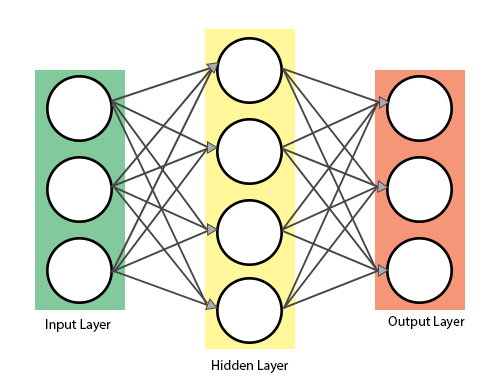
\includegraphics[width=0.6\textwidth]{common_layout}
    \caption{Common layout of a neural network.}%
    \label{fig:common_layout}
\end{figure}

\subsection{How a neural network `learns'}

For a neural network to function, it must go through a learning process, such
that it is able to sufficiently model the function it is needed for. This process
is by a set of functions $F$, where a solution $f' \in F$, and $f'$ solves
the given function best of all available solutions.

This leads to a need for a cost function, such that the best solution can be found.
A cost function is defined as a mapping from the set of functions $F$ to the real
numbers, such as:

\begin{align}
    C : F \rightarrow \mathbb{R}
\end{align}

where there exists some optional solution $f^*$, which is bound as follows

\begin{align}
    C(f^*) \le C(f) \forall f \in F
\end{align}

which means that the cost of the optimal solution is bound by the cost of
all solutions in $F$.

With this, the process of the neural network learning turns into an
optimisation problem, that is, to choose the correct weights that sufficiently
minimises the cost function $C$.

The weights are picked randomly at first, before going through a tuning
process as the network is ran. The specifics of this will depend on
the style of network and if a supervised or unsupervised learning method
is being used, which will be discussed later. Broadly, given these
initial random weights, a training process is used to tune the weights
into being suitable. An input is received, and propagates through the
network to the final output layer. Once an output is given, it may be compared
against some ground truth or metric, to evaluate if the given output was suitable.
If the output is suitable, then the next input is received. However, if this
is not the case then instead, the weights must be adjusted, such that
given the same inputs again, a more desirable result is achieved.

Commonly, this is achieved via Backpropagation. Backpropagation is the process
of calculating the required gradient, needed to adjust the weights of the
network~\cite{goodfellow2016deep}. However, this is mainly used
in supervised learning techniques, where a known value is available.

Backpropagation is achieved through repeated use of the chain rule,
to go from the output layer back to the start of the network,
using the derived gradient to update the weights in each layer,
such that they are closer to a more optimal solution.

%TODO: Expand on backprop with more refs.

\subsection{Supervised and Unsupervised learning}

As mentioned previously, there is broadly two different styles of learning,
supervised and unsupervised learning (though there is some area between,
sometimes called semi-supervised~\cite{chapelle2009semi}).

The main differences between these two are how training is conducted. In a
supervised learning environment, there exists some dataset which has an
associated set of labels, such that learning can be done and any result can
instantly be checked against this ground truth, to help the process of
backpropagation. Unsupervised learning differs to this, where a known truth
does not exist, making the process of backpropagation much harder.

Commonly, instead the result of the outcome is instead used to help the
backpropagation process, but this can also be difficult. For example,
in games the result of an action may not be seen for hundreds or thousands
of time-steps, making the process much harder~\cite{sutton1984temporal}.
This makes the learning process harder, since there is no ground truth
that can be compared against, rather a metric that will change and adapt
over a large period of time.

This can be avoided by using final results of a process, for example using the
end result of a game, rather than the score in a number of time-steps. But this
has other issues, such as slowing the learning process and potentially rewarding
unproductive behaviour that occurred as part of a game that eventually was won.
The opposite is also true, that actions that give a local reward may still lead
to failure to win the game. Because of this, it makes the learning process more
nuanced than simply comparing against a ground truth. This can be experimented
with to see how it affects learning.

\subsection{Deep Q Networks}

The main issue with using a tabular approach for keeping track of state-action
values is the number of required entries. As a more complex space needs to be
represented, the number of entries in the table would increase for every
possible combination of values. The newest approach to tackling the issue of
complex space environments is to use a neural network. The weights represent
what an expected value for a given state could be. The state is given as input
into the network and then the highest value output is chosen as an action to be
taken by the agent. The steps for running the network:

\begin{enumerate}
    \item A state is given as input into the network.
    \item The input is multiplied by the respective connected weights.
    \item The next layer is then given the input from the previous layer.
    \item The final output layer will return different values for each node in
        the layer.
    \item The node with the highest value represents the action to be taken.
    \item Once the action is taken, a reward value is recorded and used to
        update the network.
\end{enumerate}

The main difference between a Deep Q Network and a normal neural network is the
update function used. A Deep Q Network uses the loss function from the
Q-Learning algorithm to update the weights of the network. The loss function
provides a value of the target return and the predicted return. For example, the
agent could choose that in a certain state the best action would be the third
action with a value of 20. The agent takes the action and gets a returned reward
that is less. The network is then updated to return a lesser value for that
action next time the agent is in that state again. This is known as the TD
error:

\begin{align}
    TD Error = \sqrt{{(Q(s',a) - Q(s,a))}^{2}}
\end{align}

The error is the value difference between the next state reward and the current
expected reward. This tells the network whether the expected reward was correct
or far. The value is then updated by increasing or decreasing based on the
returned reward~\cite{pandey2010reinforcement}.

The update could be applied in real-time or at the end of every episode.

When using a real-time learning environment the agent is more likely to mistake
an action for being optimal from the first reward it gets. This makes the agent
tend to be more bias towards actions that get an immediate return and will not
allow the agent to see the possibilities of foreshadowing what could be a better
action in the long run. To avoid over fitting for a single environment, the
agent needs to be exposed to differing maps and states. Updating the network at
the end of each episode, may make the agent learn action pairs that are
incorrect and do not impact the reward factor. For example, the agent can move
left, which lets assume is correct, then go right and then left again. This
introduces a loop that the agent can get stuck in or an extra action step that
is unnecessary.

In order to avoid such an outcome, a discount factor $\gamma$ is used to reduce
the reward value for an incoming state. So the more steps an agent may take to
the reward, the lesser the reward value is. Once the agent takes an action,
based on the state given to the network, the reward is observed and used to
update the Q-Target. The Q-Target looks at the next state s' and checks which
action yields the highest value return. That value is then used to update the
current state in the network by using the TD Error.

\begin{align}
    QTarget = r + \gamma*Q(s',a)
\end{align}

The prediction made by the network is then subtracted according to the TD Error
equation. A learning rate is then multiplied to the value. Final update value
is:

\begin{align}
    Q(s,a) = Q(s,a) + \alpha (TDError)
\end{align}

The equation above is the same equation used in the Q-Learning algorithm. But is
implemented through the network with a gradient descent optimizer. The network
evaluates the loss function using the TD Error and then updates the relevant
weights. The learning rate $\alpha$ must be tested with multiple values. If
$\alpha$ is increased then the network may converge to an optimal value quicker
but may also tend to overshoot the local minimal and diverge from the optimal
value. This makes $\alpha$ an important hyper-parameter based on the amount of
training the agent may have. If the $\alpha$ is set to a lower value then the
agent will require more training to achieve an accurate estimate of the expected
reward for a given state action pair.

\subsection{Convolutional Neural Networks}

A Convolutional Neural Network (CNN) is a type of Artificial Neural Network
(ANN). Broadly, a CNN is similar to that of an ANN, in that it consists of a
number of neurons that have associated weights and receive some input, be that
from an input layer or another layer of neurons. Where they differ though is
that with a CNN it is assumed that the input is an image, and then because of
this, the learning procedure and design principles changes.

To give an example of why this style of network is needed, the size of a non-CNN
network must be considered. For the MNIST~\cite{lecun2010mnist} dataset, the
supplied images are $28 \times 28$. For a fully connected architecture, this
leads to $28 * 28 = 784$ weights. If an RGB image is used, this number is
multiplied by 3 to get the number of pixels in each of the 3 channels. $784 * 3$
weights is reasonable, but once moving to an image of a more reasonable size,
say $(250, 250, 3)$, the number of weights becomes very large, without even
considering the rest of the neurons in the network.

A CNN work differently however. Since it is able to assume the input is an
image, the network architecture may be built in a more specific way. That is,
instead of input consisting on a flat vector of numbers, the input may be
considered in 3D, where the images vertical and horizontal resolution make up
the width and height of the input, and the depth is made up by the channels the
image is made up of, traditionally 3. This is then helped further since the
neurons in this 3D layer are only connected to a small receptive field from the
input image, rather than the entire input like in a fully-connected network.
Broadly, it can be said that a convolutional layer takes a 3D input and
transforms it to some 3D output. In the context of the MNIST dataset, this
would be the classification. An example of this 3D network can be seen in
Figure~\ref{fig:cnn}. It can be seen that the image is given and is transformed
into a second 3D volume of the same size, but with additional channels.

The additional channels once the convolutional layer has been processed is due
to the number of filters in that layer. These are defined as the area the
neuron in a given layer connects to. For example a neuron in the first layer
may look at a $3 \times 3$ section of the input, extending across all channels
of the input. This filter is applied to the entire image by moving it over every
pixel combination it fits on, and at each location the dot product on the input
and the values in the filter is computed. For the whole image $I$ and a filter
$F$, this is defined as follows:

\begin{align}
    {(I*F)}_{xy} = \sum^{h}_{i=1} \sum^{w}_{j=1} F_{ij} \cdot I_{x+i-1, y+j-1}
\end{align}

which means that for a given a $(x,y)$ position, the value of the filter at that
point for a given filter is the dot product of each value in the input and the
value in the filter.

These filters are stacked, which then increases the receptive field of the later
layers. This process was mirrored on features found in
biology~\cite{hubel1968receptive}. The receptive field refers to the area that a
given neuron is receiving input from. For the first layer, this is simply the
size of the filter, for example the $3 \times 3$ grid. However, this layer is
then used as input for the next layer. It can be said that the second layer's
receptive field relative to the image for a filter of size $3 \times 3$ is
5. This increases throughout the network, building up evermore complex and
abstracted representations of the image, that are increasingly global across the
image. This can be seen in the filters that are calculated in the network,
where the earlier layers contain low-level features, where the later
ones become more abstract and cover larger parts of the image,
as shown in Figure~\ref{fig:filter_example}.

In general, the formula a given layer $l_k$, the receptive field can be
calculated as follows:

\begin{align}
    l_k = l_{k-1} + ((f_k - 1) * \prod_{i=1}^{k-1}s_i)
\end{align}

where $f_k$ is the filter size of layer $k$ and $s_i$ is the stride for the
$i^{th}$ layer.

%TODO: Read over and check, but should be done now.

\begin{figure}
    \centering
    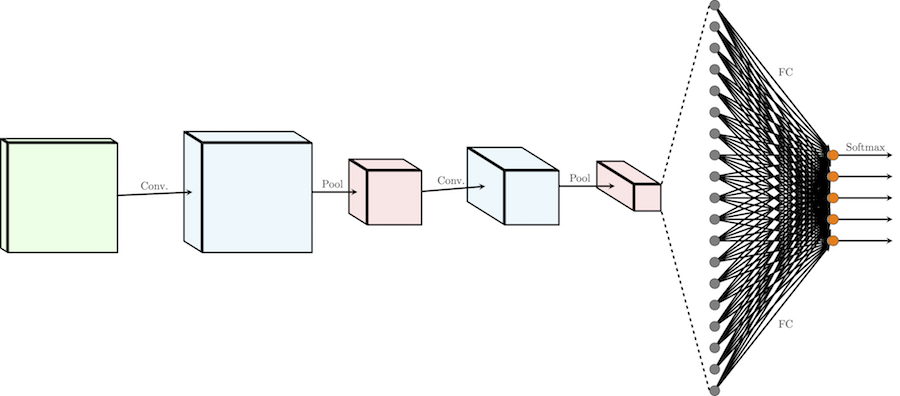
\includegraphics[width=0.9\textwidth]{cnn}
    \caption{Common layout of a convolutional neural network, from
    Cambridge Spark\cite{cnn-layout}.}%
    \label{fig:cnn}
\end{figure}

\begin{figure}
    \centering
    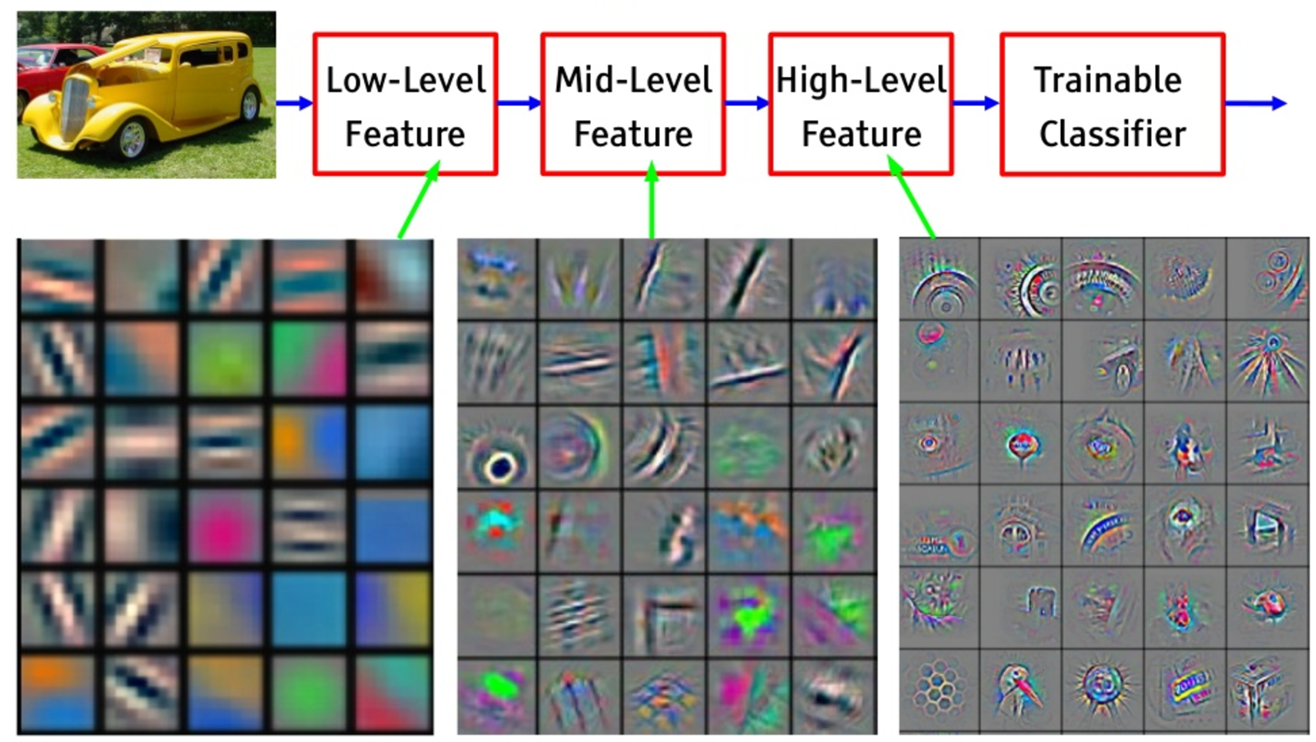
\includegraphics[width=0.9\textwidth]{filter_example}
    \caption{Examples of filters from various layers, from
    NIPS'2015 Tutorial\cite{filterexample}.}%
    \label{fig:filter_example}
\end{figure}

\subsubsection{Other required techniques}

There are other techniques that go alongside a CNN by default, and have been
mentioned previously. This includes both pooling layers and the concept of
striding which is used both in the pooling layer and also the convolutional
layer.

When a filter uses a stride, the filter is moved by more than a single pixel
each time. By default a stride is 1, that is it is applied to every single pixel
on the input. However, it is also common to have a stride of two, or in some
rare cases, a stride of greater than 2. When this is the case, the filter
is moved two pixels at a time, rather than 1. This leads to less overlap in the
receptive fields, but does have the potential downside of reducing the
resolution of the input.

A pooling layer is a form of down-sampling. Given an input the pooling layer
will reduce the resolution of it in some fashion. The most common pooling layer
used is the max-pooling layer. This layer takes the maximum value in a filter
and uses that as the value for that filter. This is commonly done with a filter
of size $2 \times 2$ and a stride of 2. This results in an image that is halved
in both the width and height dimension. This is useful to help reduce the number
of parameters in a given network, so is commonly applied after each
convolutional layer. An example of a max-pooling layer can be seen in
Figure~\ref{max_pool}.

\begin{figure}
    \centering
    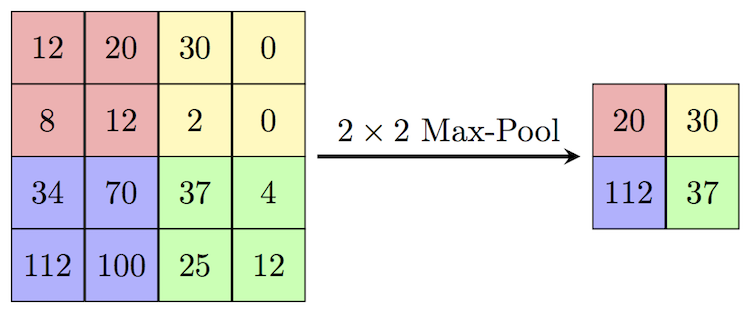
\includegraphics[width=0.9\textwidth]{max_pool}
    \caption{Example of max-pooling, from Computer Science Wiki\cite{max_pool}.}%
    \label{fig:max_pool}
\end{figure}

\section{Challenges}
% Add more info here about the tech and the challenges it faces
% i.e. the problems in Reinforcement Learning as a whole

\section{Reinforcement Learning For Games}
% The earlier sections should cover the general tech,
% whereas this section will talk about it applied to games
% and the unique problems that raises.

%TODO: Add differences between supervised and unsupervised.
%Include about using replays.

\section{Existing Methods}
% This should then move on from the previous section
% to show how the outlined challenges are dealt with.

\section{Conclusion}
% Conclusion of the research and what it means moving into the
% implementation and evaluation.
